\newpage
\section{Testing}

A build methodology was used to explore the feasibility of proposed system. After implementation, viability of the solution was tested by simulating updates to a development version of the firmware running on a prototype board.

\subsection{Implementation details}

A set of Python scripts aids with function compilation and packaging. Functions are discovered and allocated by searching function definitions from all source files. Global variables are extracted from symbol tables after all object files are compiled. Reason for this difference is that argument types must also be know about functions. Data about functions and global variables, along with respective object codes, gets stored in a SQLite3 database. Scripts also exist for generating interception macros, linker script, and packages with headers.

Function table can not be implemented as branch table, as internal Flash and \gls{sram} are too far away in the memory space. Function table will therefore contain pointers, 4 bytes per function. Storing 3 bytes per function would require 2 instructions of additional overhead per function call, so it has been decided that 4 bytes per function will be stored (Appendix \ref{apx:calls}). Pointers will point to the first instruction of the function (right after the header).

Firmware contains a table generation function (Appendix \ref{apx:gentable}) that must run before any application software gets called. It starts walking package headers from the beginning of space allocated for such packages, jumping over function bodies based on length, and stops on the first header with the type 'nothing' (\texttt{0xff}, table \ref{tab:header}). Function pointers are added to the function table, and global variables get copied to their respective allocated memory areas.

\subsection{Function discovery and preparation}

Aforementioned Python scripts were tested against simple test functions, as well as \gls{aocs} repositories. For discovering global variables, two methods were compared: parsing source code variable definitions, and compiling source with \texttt{-fdata-sections} to discover global variable names from symbol table. Former method was not sufficiently effective due to large amount of different global variables, including matrices and other complex types. Using the latter method, most functions and all global variables were successfully packaged.

As one limitation, the proposed solution does not allow the packaging of functions with a variable number of arguments, for example, \texttt{sprintf}. It remains unsolved, how to typedef a function pointer to function with variable number of arguments.\todo{look at it one more time}

\subsection{Running application functions}

\subsubsection{Fully self-contained function}

As the first test, a fully self contained function was written, meaning one that did not depend on any external variables or functions, including any standard library or operating system methods. This function blinked a \gls{led} by writing appropriate values directly to the \gls{mcu} registers.

It was compiled independently of the rest of the firmware and tested without any issues. A minor inconvenience was noted: debug symbols for applications functions are not available to the debugger from the firmware's \gls{elf}.

\subsubsection{Calling firmware functions}

Next, a function was written that blinks \glspl{led} by calling respective \gls{hal} methods. Several issues arouse, all of which were possible to mitigate, so that this test was also mostly successfully concluded.

Firstly, author was unable to find any way to tell GNU linker \texttt{ld} to use symbol addresses from a map file generated by prior linking. Even though \textcite{Dunkels2006} claims to have used just the map file for pre-linking, documentation, different online sources nor a online forum (\url{https://stackoverflow.com/q/48028126/7088748}) had revealed any information on the matter by the time of writing. This resulted in the need to link firmware separately once, and then again with each application function, hoping that firmware layout stays unchanged. Initially that was not the case, but after explicitly specifying section order in linker script, layout consistency was achieved.

Secondly, issues arouse with the way GNU C compiler handles local constants. \Gls{hal} functions for accessing \gls{gpio} take a struct of port and pin as an argument. Unfortunately, compiler placed the structs to \texttt{.rodata} section separately from the function code, even though they were local. Even when placing function's \texttt{.text} and respective \texttt{.rodata} containing only function's local constants side by side with linker, compiler has already generated code that expects to use absolute memory addresses. More about that issue can be found in section \ref{s:rodata}. For the purpose of this test, the issue was mitigating by storing all pin-s and ports to single-byte local variables, that the compiler decided to store directly within the code section.

\subsection{Performance}

Performance overhead per function call with the implemented system is $3$ instructions. Storage overhead per function is $12$~B.

An in-progress \gls{aocs} library was packaged, and results analyzed. The average size of compiled functions was $533~\text{B}\ (s=1201~\text{B})$ (figure \ref{fig:kalman}). Largest function was just over $8.5$~kB. However, the library also contained several extremely small functions (for example appendix \ref{apx:cos} just $28$~B) which would not stay as separate functions in later versions.

Overall storage overhead for the specific version tested was $2.25\%$. For aforementioned reasons the actual overhead would probably be lower.

\begin{figure} [htb]
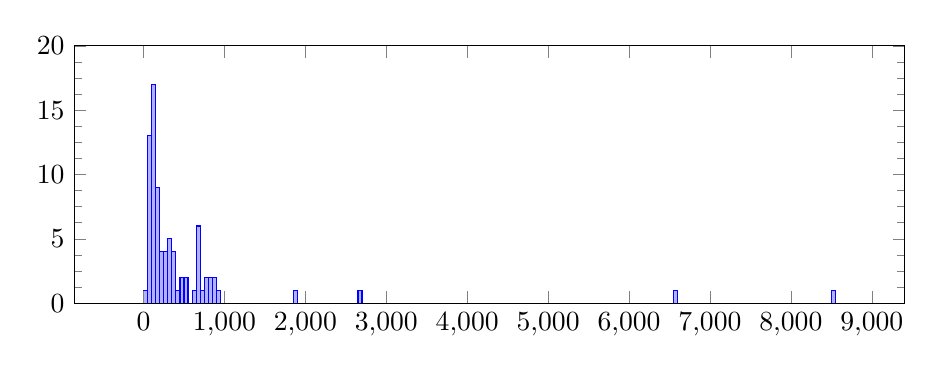
\begin{tikzpicture}
\begin{axis}[
    ymin=0, ymax=20,
    minor y tick num = 3,
    area style,
    width=\textwidth,
    height=0.4\textwidth
    ]

\addplot+[ybar interval,mark=no] plot coordinates { (0, 1) (50, 13) (100, 17) (150, 9) (200, 4) (250, 4) (300, 5) (350, 4) (400, 1) (450, 2) (500, 2) (550, 0) (600, 1) (650, 6) (700, 1) (750, 2) (800, 2) (850, 2) (900, 1) (950, 0) (1850, 1) (1900, 0) (2650, 1) (2700, 0) (6550, 1) (6600, 0) (8500, 1) (8550, 0) };
\end{axis}
\end{tikzpicture}
\caption{Histogram of sizes of compiled functions from a in-progress \gls{aocs} library.}
\label{fig:kalman}
\end{figure}

\TODO{You could compare an artificial partial firmware update. Full firmware update vs. your method - how much data is sent to the spacecraft and how long it would take to write it in Flash. Flash writing speed can be calculated from the MCU datasheet.}

\subsection{Section .rodata}\label{s:rodata}

ESTCube is using GNU Tools for Arm Embedded Processors (version 7.2.1 at the time of writing) to compile \gls{obc} software. When the GNU C compiler finds local constants that are longer than a byte, it separates them from the code, and creates a \texttt{.rodata} section for them. The \texttt{.text} section will then contain relative reference (\texttt{//1}) to an absolute address (\texttt{//2}) inside the \texttt{.text}, which in turn points to the data (\texttt{//3}) inside \texttt{.rodata} (figure \ref{fig:rodata}). This structure remains even when linker is told to put \texttt{.text.function} and corresponding \texttt{.rodata} into single output section.

\begin{figure} [htb]
\begin{lstlisting}[language=C]
int function() { int a[] = {97, 98, 99, 100, 101, 103}; }
\end{lstlisting}
\begin{lstlisting}[style=asm]
// Undesirable:
0000 <.text.function>:
/---/
6:  4b07    ldr     r3, [pc, #28] ; (24 <function+0x24>) //1
/---/
24: 0000    .word   0x0000 //2 absolute address of .rodata, currently not linked
0000 <.rodata>: // absolute address will be replaced by linker
0:  0061    .word   0x0061 //3
4:  0062    .word   0x0062
8:  0063    .word   0x0063
c:  0064    .word   0x0064
10: 0065    .word   0x0065
14: 0067    .word   0x0067
\end{lstlisting}
\caption{Local constants after compilation with GNU C compiler}
\label{fig:rodata}
\end{figure}

Even when using \gls{pic}, code uses expressions relative to the \gls{pc} to access the \gls{got}, but \gls{got} still contains absolute memory addresses to \texttt{.rodata}. However, in all cases, absolute memory addresses to application function components, even when in the \gls{got}, are undesirable, because by requirements, code should not require on-board modifications and should be movable in memory space.

Research on documentation, an online forum (\url{https://stackoverflow.com/q/45371949/7088748}) and the compiler support mailing list (\url{https://gcc.gnu.org/ml/gcc-help/2018-03/msg00015.html}) had not revealed any potential solutions by the time of writing.

This is not a fundamental problem with the proposed approach, since the compiler is already storing data (absolute memory addresses in this case) at the end of the \texttt{.text} section, and referencing it by \gls{pc}-relative expressions. The local constants could be stored the same way. Instead, this is a problem since nobody has happened to implement a compiler flag for such behavior, most likely due to lack of use cases prior to this work.
